%!TEX encoding = UTF-8 Unicode
%!TEX program = xelatex

% 全局字体默认是 11pt
% compress 选项可以压缩 outer 元素的占用空间
% hyperref 中如果选择 colorlinks=true 会导致所有链接都变色
% dvipsnames,svgnames,x11names 都是 xcolor 的选项,只是多一些颜色选择
\documentclass[UTF8,14pt,aspectratio=43,dvipsnames,svgnames,x11names,hyperref={urlcolor=blue}]{beamer}  

% 中文包,ctex 封装了 xeCJK
% window 系统把 fontset 参数改为 windows,或者依然是 none 
% 目前 mac 系统的 fontset 参数还有 mac; macold; macnew。 都可以顺利编译,具体区别不明,可以参考 ctex github 项目的有关 issue
\usepackage[UTF8,fontset=none]{ctex}
\usepackage{amsmath}

% 图片包
\usepackage{graphicx}
\usepackage{tikz}

% 表格包
\usepackage{booktabs}
\usepackage{longtable}

% 引用包
% biblatex 最现代(默认后端使用 biber),但不一定被期刊接受。比较传统的有 bibtex 和 natbib。
% 注意很可能需要根据编辑器配置编译流程,可参考 tex stack exchagne 上的问答
% 各参数可以选择各种格式,参考投稿要求和 overleaf 教程
% style 为文后列表格式,citestyle 为文内引用格式
% sortlocales=zh__pingyin 能使中文引用列表按一作姓氏首字拼音排序。
\usepackage[style=gb7714-2015,citestyle=authoryear-comp,sorting=ynt,sortlocale=zh__pinyin]{biblatex}

\renewcommand{\arraystretch}{1.2} % default is 1.0 避免表格内容上沿离边界太近,特别是汉字

\usetheme{lingnan}  % 指定全局模板主题
\usefonttheme[onlymath]{serif}  % 数学字体

% 指定中文字体
% 如果使用了系统中没有的字体会报错
% mac 系统下 ctex 包无论采用哪一个 fontset 参数都会引起一些警告,但仍然可以顺利编译
\setCJKmainfont[BoldFont={HiraginoSansGB-W6},ItalicFont={HiraginoSansGB-W3}]{HiraginoSansGB-W3}
\setCJKsansfont{HiraginoSansGB-W3}
\setCJKmonofont{NotoSansMonoCJKsc-Regular}
\XeTeXlinebreaklocale “zh”  % 中文断行

% 设定新字体的快捷命令,可以在局部改用这些预设字体
\setCJKfamilyfont{songti}{STSongti-SC-Regular}
\newcommand{\ST}{\CJKfamily{songti}}
\setCJKfamilyfont{kaiti}{STKaitiSC-Regular}
\newcommand{\KT}{\CJKfamily{kaiti}}

% 指定默认图片目录
\graphicspath{{./img/}}

% 指定参考文献 bibtex 文件
% cnki 无法直接导出 bibtex 格式,可以通过 endnote 等工具转换
\addbibresource{ref.bib}

% 设定目录深度,只到第 1 级
\setcounter{tocdepth}{1}

% 开启图标编号
\setbeamertemplate{caption}[numbered]

\setbeamerfont{date}{size=\small}

% 基本信息,这些要写在 titlepage 前面作为 preamble
\title[short title]{long title}
\subtitle[short subtitle]{long subtitle}
\institute[short institute-name]
{
	\inst{1}	
	long institute-name 1
	\and
	\inst{2}
	long institute-name 2
}
\author[short author-name]
{
	long author-name 1\inst{1}
	\and
	long author-name 2\inst{2}
}
\date[\today]{\today}
\titlegraphic{
\includegraphics[width=0.5\textwidth]{logo3.png}}

\begin{document}

% 标题页,根据 preamble 的基本信息生成。前后不用 \begin{frame} \end{frame} 包覆也能生成,好像没什么区别
% plain 选项可以取消当前页的 headline, footline, 以及 sidebar
\frame[plain]{\titlepage}

% 目录页
% 标题可以用 \frametitle 也可以跟在 \begin{frame} 后面作为参数
\begin{frame}\frametitle{Outline}
	% toc 有 pausesections 选项会生成等于 section 数量的页数,各个 section 按顺序增量出现,一般用不上。
	% 还有个 part=1 的选项控制目录深度?
	\footnotesize
	\tableofcontents  % 数量过多时要自己控制字体大小才能完全显示
\end{frame}

% 声明一个 section,注意观察在不同主题的导航栏中显示的效果
% section 的声明也不影响其内外 frame 的结构和呈现 
\section{列表}

\subsection{基本列表} % 同样注意观察子节在导航栏中的效果
	%  frame 为常规“页”,但也可以通过 pause 等方式在一个 frame 定义内实际生成多张 slides
	% [ ]内选项,默认为 c-中央对齐,还可以有 t-上部对齐, b-底部对齐
	\begin{frame}[t]{无序列表}  
	\begin{itemize}
		\item The first item
		\item The second item
		\item The third item
		\item The fourth item
	\end{itemize}
	\end{frame}


	\begin{frame}{有序列表}
		\begin{enumerate}
			\item The first item
			\item The second item
			\item The third item
			\item The fourth item
		\end{enumerate}
	\end{frame}

\subsection{描述列表}
\begin{frame}{描述列表}
	\begin{description}
		\item[First Item] Description of first item
		\item[Second Item] Description of second item
		\item[Third Item] Description of third item
		\item[Forth Item] Description of forth item
	\end{description}
\end{frame}

\section*{不进入目录的节} % 加星号就不会进入目录

\section[文本字符]{文本字符}  % 方括号中的 short title 选项才是进入导航栏的
\begin{frame}{各类变体}
	\emph{Sample Text} \\
	\textbf{Bold} \\
	\textit{Italic} \\
	\textsl{Slanted} \\
	\alert{Aleart} \\
	\textrm{Roman} \\
	\textsf{SansSerif} \\
	\textcolor{green}{Color} \\
	\structure{Structure}	\\
	\ST 宋体\\
	\KT 楷体
\end{frame}

\begin{frame}[fragile]{逐字符输入}  % 要使用 verbatim 必须在有 fragile 选项的 frame 里
	% 注意下面的写法会连空格和制表符也显示出来
	% 另外还存在有 semiverbatim 环境
	\begin{verbatim}
		Sample text
	\end{verbatim}
\end{frame}

\section[帧内结构]{帧内结构}
\begin{frame}{分栏与子页}
	\begin{columns}
		\column{.5\textwidth}  % 宽度可调
			First column text and/or code
		\column{.3\paperwidth}
			Second column text and/or code
	\end{columns}
\end{frame}

\begin{frame}{块}
	\begin{columns}
		\column{.5\textwidth}
			\begin{block}{Beamer 内建区块环境}
				block 普通环境\\
				theorem 定理环境\\
				lemma 引理环境\\
				proof 证明环境\\
				corollary 推论环境\\
				example 示例环境\\
				alertblock 警示环境
			\end{block}
		
		\column{.5\textwidth}
			% 注意定理名称为中括号而非花括号包覆,且 theorem 环境的标题会有“定理”开头
			\begin{theorem}[勾股定理]
				% 使用 equation 环境会有公式编号,直接用 $ $ 的环境则没有
				\begin{equation}  
					a^2+b^2=c^2
				\end{equation}
			\end{theorem}
	\end{columns}
\end{frame}

\subsection{数学公式}

\begin{frame}{数学公式(非编号)}
	行内公式 $e^{ix}=cosx+isinx$\\
	代码块形式
	$$e^{ix}=cosx+isinx$$
	以上两者均不编号
\end{frame}

\begin{frame}{数学公式(编号)}
	\begin{block}{equation 环境}
		% equation 后加*则不编号
		\begin{equation} \label{euler eqn}
			e^{ix}=cosx+isinx
		\end{equation}
	\end{block}
	\begin{block}{嵌套split,注意可以逐行编号也可以整体编号}
		\begin{equation}
			\begin{split}
				A & = \frac{\pi r^2}{2} \\
				& = \frac{1}{2} \pi r^2
			\end{split}
		\end{equation}
	\end{block}
\end{frame}

\begin{frame}{数学公式(编号)}
	使用 equation, split, multline, align, gather 环境,默认编号。环境声明加星号后缀则不编。\\
	引用需要用 label 标签后再使用 eqref/ref。\\
	如: \eqref{euler eqn} 式
\end{frame}

\begin{frame}{子公式编号}
	\begin{subequations}
	% subequations 环境下属 label 内小写字母后缀为特别二级排序
	% \notag 则为不编号
		\begin{align}
			y5=x5+z5 \label{Za}\\
			y6=x6+z6 \notag \\
			y7=x7+z7 \label{Zb}
		\end{align}
	\end{subequations}
	Next equation:
	\begin{equation}
		y8=x8+z8 \label{WW}
	\end{equation}
\end{frame}

\section[表格与图片]{表格与图片}
\begin{frame}{表格}
	\begin{table}[t]  
	% 参数,似乎在 Beamer 中无效
	% h - here
	% t - top
	% b - bottom
	% p - special page
		\centering
		\caption{Caption here\label{tab:tablename}}
		% tabular 环境的 l|cc 参数就是逐列声明对齐方式,第一列和第二列之间加上竖线
		% \hline 为水平线
		\begin{tabular}{l|cc} \hline  
			\textbf{column 1} & \textbf{column 2} & \textbf{column 3} \\ \hline
			Hello & Beamer & NAN \\ \hline
			$\alpha+\beta$ & $\gamma+\eta$ & 34\% \\ \hline
		\end{tabular}
	\end{table}
\end{frame}

\begin{frame}[allowframebreaks]{跨页表格}
	表格代码生成网站 https://www.tablesgenerator.com/
	\begin{longtable}[c]{@{}llr@{}}
		\toprule
		\multicolumn{2}{c}{Item} &            \\* \midrule
		\endfirsthead
		%
		\multicolumn{3}{c}%
		{{\bfseries Table \thetable\ continued from previous page}} \\
		\toprule
		\multicolumn{2}{c}{Item} &            \\* \midrule
		\endhead
		%
		\bottomrule
		\endfoot
		%
		\endlastfoot
		%
		Animal     & Description & Price (\$) \\* \midrule
		Gnat       & per gram    & 13.65      \\
				   & each        & 0.01       \\
		Gnu        & stuffed     & 92.50      \\
		Emu        & stuffed     & 33.33      \\
		\pagebreak  %手工指定比较好
		\toprule  %手工重复表头
		\multicolumn{2}{c}{Item} &            \\* \midrule
		Animal     & Description & Price (\$) \\* \midrule
		Pig        & hot         & 44.22      \\
		Cow        & cold        & 22.33      \\
		Armadillo  & frozen      & 8.99       \\* \bottomrule
		\end{longtable}
\end{frame}

\begin{frame}{图片}
	\begin{figure}[tb]
		\centering
		
\includegraphics[width=0.9\textwidth]{logo2.png}
		\caption{Caption here\label{fig:figure1}}
	\end{figure}
\end{frame}

\begin{frame}
	% 通过 tikz 可以对图片进行各种深入操作
	% 比如这里挤满页面左侧 padding 的插入图片
	\begin{tikzpicture}[remember picture, overlay] % 在前面的图片上做覆盖,标准的水平居中全页宽图片显示,可能需要多编译几次
		\node[overlay,inner sep=0pt,outer sep=0pt,anchor=west] at (current page.west){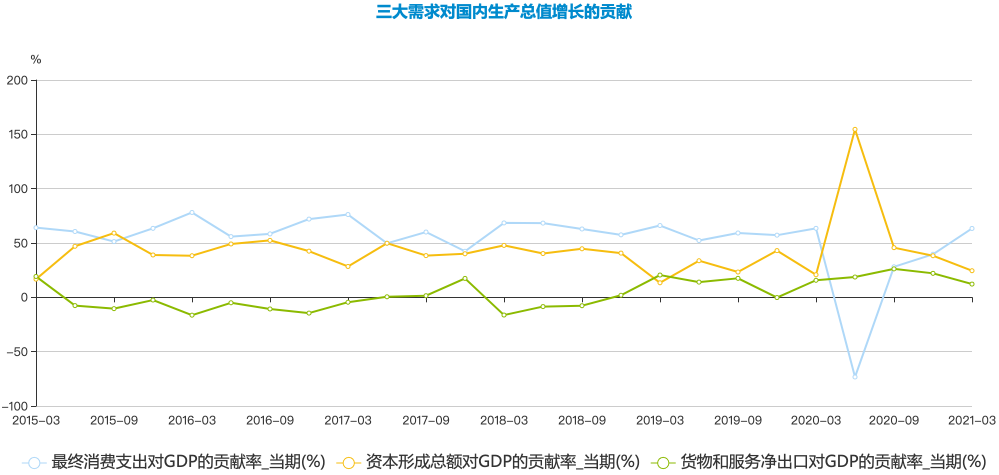
\includegraphics[width=\paperwidth]{三大需求对国内生产总值增长的贡献.png}};
	\end{tikzpicture}
\end{frame}

\section[对齐与空格]{对齐与空格}
\begin{frame}{文本对齐}
	\begin{center}  % 还有 left,right
		居中对齐文本
	\end{center}
\end{frame}

\begin{frame}{文本空格}
	some \hskip20pt text here  % 还可以有 vskip 垂直空格,负的 pt 可以缩减间距,单位也可以用 cm,ex,em 等等
\end{frame}

\section[Overlay 蒙板覆盖]{Overlay 蒙版覆盖}
\subsection[暂停]{暂停}
\begin{frame}{暂停}{pause}
	% 使用 \pause 来分割,和目录页中的 pausesection 选项一样会生成多张 slide
	\textbf{Step 1:} Compute the maximal suffix of $w$
	with respect to $\preceq_l$ (say $v$) and the
	maximal suffix of $w$ with respect to $\preceq_r$
	(say $v’$).\\
	
	\pause
	
	\textbf{Step 2:} Find words $u$, $u’$ such that
	$w = uv = u’v’$.\\
	
	\pause
	
	\textbf{Step 3:} If $|v| \le |v’|$, then output
	$(u,v)$. Otherwise, output$(u’,v’)$.
\end{frame}

\subsection[显式声明]{显式声明}
\begin{frame}{显式声明}
	% The specification <1-> means “display from slide 1 on.” <1-3>
	% means “display from slide 1 to slide 3.” <-3,5-6,8-> means
	% “display on all slides except slides 4 and 7.”
	用尖括号 <> 内的数字声明,更适合于多个项目按不同页面划分不同的效果
	\begin{itemize}[<+->]  %: If you want each item of a list to appear in order, use the [<+->] option?
		\item<1> $abcadcabca$\\
		\item<1-2> $abcabcabca$\\
		\item<1-2> $accaccacca$\\
		\item<1> $bacabacaba$\\
		\item<1,3> $cacdaccacc$\\
		\item<1-2> $caccaccacc$
	\end{itemize}
\end{frame}

\begin{frame}{显式声明的另一个用途}
	可以用在命令的执行上  % 还有 text,color 等命令都可行
	\vskip12pt
	\alert{Alert on all slides}\\
	\alert<2>{Alert on slide 2}\\
	\alert<3>{Alert on slide 3}\\
	\alert<1,3>{Alert on slides 1 and 3}\\
	\alert<-2,4>{Alert on slides 1, 2 and 4}
\end{frame}

\subsection[其他相关用途]{其他相关用途}
\begin{frame}[fragile]{其他有用的 Overlay 方法}
	\begin{verbatim}
\onslide<1,2>
\only<1,2> 
\visible<1,2>
\invisible<1,2>
\alt<1,2> 
\temporal<1,2>
\uncover<1,2> 
\end{verbatim}
\end{frame}

\begin{frame}{区块应用}
	区块环境同样可用
	\begin{theorem}<1->
		There exists an infinite set.
	\end{theorem}
	\begin{proof}<2->
		This follows from the axiom of infinity.
	\end{proof}
\end{frame}

\section[超链接]{超链接}
\subsection[内部链接]{内部链接}
\begin{frame}[label=内部链接]{内部链接}
	点击按钮跳转 \hyperlink{内部链接目标}{\beamergotobutton{Detail}}\\
	$\backslash$hyperlink 的 target name 参数需要在 frame 的 label 选项中指定并对应调用
\end{frame}

\begin{frame}[label=内部链接目标]{内部链接目标}
	点击按钮回到先前页面 \hyperlink{内部链接}{\beamerreturnbutton{Return}}
\end{frame}

\subsection[外部链接]{外部链接}
\begin{frame}{外部链接}
	- 显式 \url{www.baidu.com}\\
	- 隐式 \href{www.baidu.com}{百度}\\
	问题是 hyperref 中一旦启用 colorlinks,就要指定除 urlcolor 外的 linkcolor,filecolor,citecolor 等以保持颜色风格与主题一致。所以如非必要,不要放外部链接
\end{frame}

\section{引用}
\begin{frame}{引用}
	\footnotesize
	注意编译时要选择所使用包(如 biblatex)对应的后端(如 biber)\\
	另外文内引用的年份位置会生成可点击的超链接\\
	~\\
	这里使用的citestyle=authoryear-comp\\
	~\\
	几种不同的引用方式:
	\begin{itemize}
		\item cite 没括号:\cite{mincer1962job}
		\item textcite 年份有括号:\textcite{schultz1961investment}
		\item parencite 整体括号:\parencite{孟望生2018人力资本统计核算方法研究述评,李海峥2010中国人力资本测度与指数构建}
		\item fullcite 整体引用:\fullcite{李海峥2010中国人力资本测度与指数构建}
	\end{itemize}
\end{frame}

\begin{frame}{参考文献}
	\AtNextBibliography{\scriptsize} % 不可以直接用 \scriptsize 改变参考列表字体大小
	\nocite{*} % 不管文中有没有正是引用,后续参考列表均列出全部 .bib 文件中的参考文献
	\printbibliography % 此命令会自动生成一个名为“参考文献”的 section 和 frame,但不会生成 frametitle
\end{frame}

\end{document}